% -*- Mode: LaTeX; Mode: Flyspell -*-

\section{Introduction}

\paolo{
The provenance of data is a form of structured metadata that records the processes involved in data production. In addition to references to data generation or transformation processes, a \textit{provenance trace} typically includes input  or intermediate data products as well as references to \textit{agents}, that is the humans or software systems who were responsible to enact those processes.
%
	In multi-party collaboration settings that involve data sharing, as well as in third party auditing of data and processes, there is a broad expectation that 
shipping the available provenance to collaborators, or more generally publishing it along with the data, may help data consumers, including auditors, form judgements regarding the reliability of the data itself.
}

%
\paolo{
	Offering to disclose the provenance of  data as evidential basis for establishing data quality and reliability is particularly important when data products are exchanged as part of transactions that involve parties with limited mutual trust. 
This is the case for instance of \textit{dynamic coalitions}~\citep{BFJM06}, ad hoc collaborative partnerships that are created 
to pursue a common goal, in scenarios such as multi-agency emergency/threat responses, as well as the exchange of intelligence information. 
Despite the need to share data of a possibly sensitive nature, these coalitions are characterized by a lack of established interaction protocols and by limited trust amongst the partners. 
}
\paolo{
This situation creates a tension between data providers and consumers, when it comes to negotiating the level of detail of the provenance that providers are prepared to offer to consumers. 
On the one hand, consumers will require as much provenance detail as possible, to use as a basis for establishing data credibility.
Data providers, on the other hand, will be reticent to offer detailed provenance traces, because those may contain sensitive information regarding their own internal processes as well as any proprietary data used by those processes. 
%
In fact, the provenance of a data product will typically contain more sensitive information than then data product itself.}


\paolo{\subsection{Motivating scenario: provenance of intelligence information}
	%
To appreciate how such tension may arise, consider a scenario where a public agency PA  wants to buy intelligence reports, say about potential threats to the public, from an intelligence provider, IP.
%
Under assumption of limited trust, PA will want to mitigate the risk of acting upon information provided by IP, which is potentially unreliable. 
% 
At the same time, IP has a business incentive to supply PA with additional evidence that facilitates PA's risk assessment and thus increases the chance of a successful transaction.}

%
\paolo{The  key assumption that motivates our work is that the provenance of each intelligence report is relevant in contributing, at least in part, the required evidence. 
%
A fictional but realistic example of provenance for an intelligence report such information is shown in Fig.~\ref{fig:graph-example}.
%
Provenance can be visually depicted as a digraph whose nodes represent either \textit{entities} (ovals in the figure), i.e., data, documents, etc., \textit{activities} (rectangles), which represent the execution of some process over a period of time, or \textit{agents} (pentagons), which represent  humans or computing systems. 
%
The edges represent various types of directed relationships, the most common being ``activity $a$ used entity $e$'', ``entity $e$ was generated by activity $a$'', ``activity $a$ was associated with agent $ag$'' (i.e., $ag$ was responsible for $a$), and more.
it is also possible to annotate each of the nodes using either pre-defined properties, as defined by the PROV standard, or user-defined properties, for instance to qualify the kind of data and activities involved in the process execution. We omit annotations from our examples for readability, and because they are not handled \jwb{within this work}  in any special way.}

\paolo{Formally, such a graph is a depiction of a PROV document, which in turn conforms to the W3C PROV data model~\citep{w3c-prov-dm}, introduced in Sec.~\ref{sec:prov-core}. 
We will use the graph representation of provenance throughout the paper, as it facilitates reasoning about the mechanisms for provenance abstraction, which are at the core of our work.
The graph layout in \jwb{Figs.~\ref{fig:graph-example},~\ref{fig:graph-example-abs-1} and \ref{fig:graph-example-abs-2}} is such that the process execution flows from top to bottom, i.e, the top entities represent initial inputs, while the outputs are at the bottom.
}



\begin{figure*}
	\begin{center}
		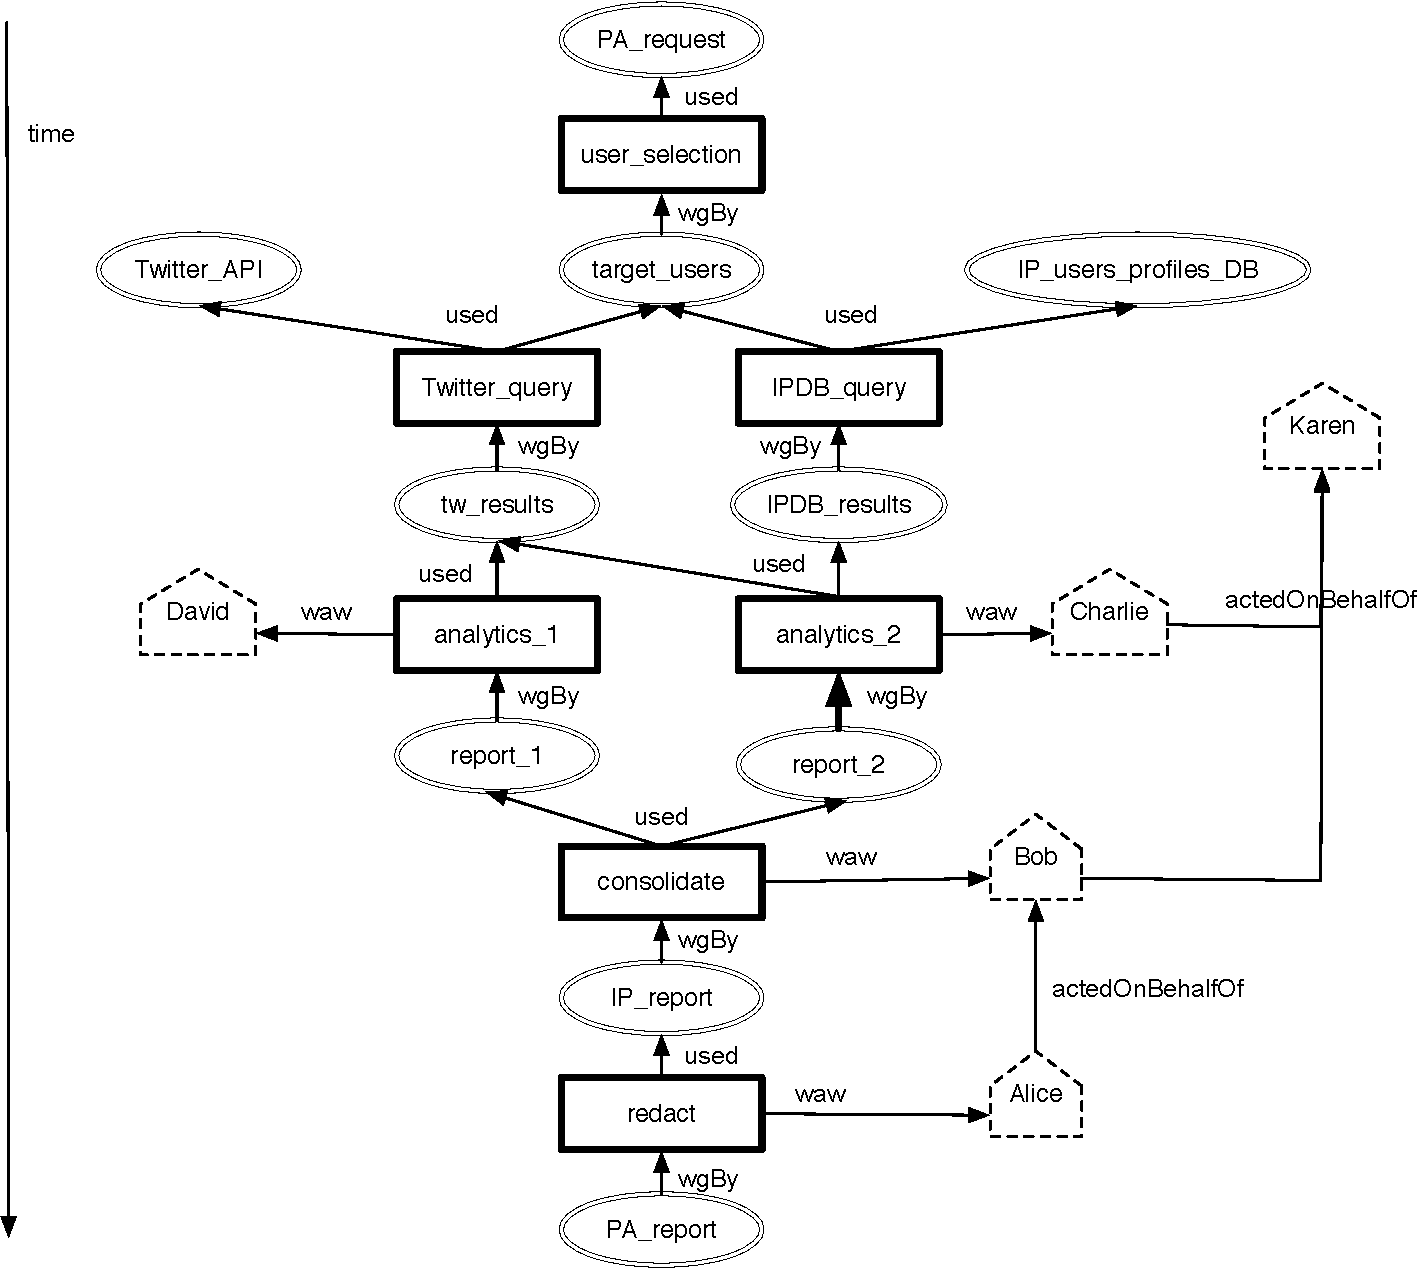
\includegraphics[width=.7\textwidth]{figures/analytics-ex-baseline-FGCS-paper}
		\caption{Example provenance graph depicting the generation of an intelligence report}
		\label{fig:graph-example}
	\end{center}
\end{figure*}	

\paolo{
%
This provenance graphs depicts a process of intelligence report generation, which is initiated by a request by PA. 
The process identifies target users from the request and acquires further information about those users, both on Twitter (\texttt{Twitter\_query}) and from a proprietary database, \texttt{IP\_users\_profile\_DB}.
%
The results are fed to two analytics sub-processes, each of which generates a report. 
%
Note that \texttt{analytics\_1} only uses Twitter data, while \texttt{analytics\_2} also uses query results of the proprietary database.
A \texttt{consolidate} step follows, which produces a master \texttt{IP\_report}.
This is checked, presumably to validate and possibly also to remove sensitive information, before the final \texttt{PA\_report} is generated for the customer.
%
Notice that various agents are specified as being responsible for some of the steps, along with their chain of responsibility, i.e., \texttt{Alice} acts as \texttt{Bob}'s delegate, who in turn reports to \texttt{Karen}, along with \texttt{Charlie}}.


\paolo{As we can see, the full-fledged provenance graph contains information about IP's internal business processes, including the use of a proprietary database, which IP may consider privileged.
It is therefore realistic to imagine that IP may want to  obfuscate some of those elements. 
Using our selective disclosure model, IP marks the sensitive elements, in this case the \texttt{redact} activity as well as the references to the two analytics processes. Note that doing so does not require any knowledge of the graph topology, rather only of the nodes (either activities or entities) that are to be abstracted out.}

\paolo{It is important to note that the PROV document represented in Fig.~\ref{fig:graph-example} is \textit{valid}, in the sense that it satisfies all the constraints specified as part of the PROV standard~\citep{w3c-prov-constraints}.
As we will see in the rest of the paper, replacing the three selected nodes with a single abstract node (an activity in this case) while preserving the validity  of the document, i.e., while complying with the PROV constraints, requires that all other nodes that lie on the directed paths that connect these nodes are also removed. 
In this example, the result of such abstraction operation is shown in Fig.~\ref{fig:graph-example-abs-1}.
}

	\begin{figure*}
		\begin{center}
			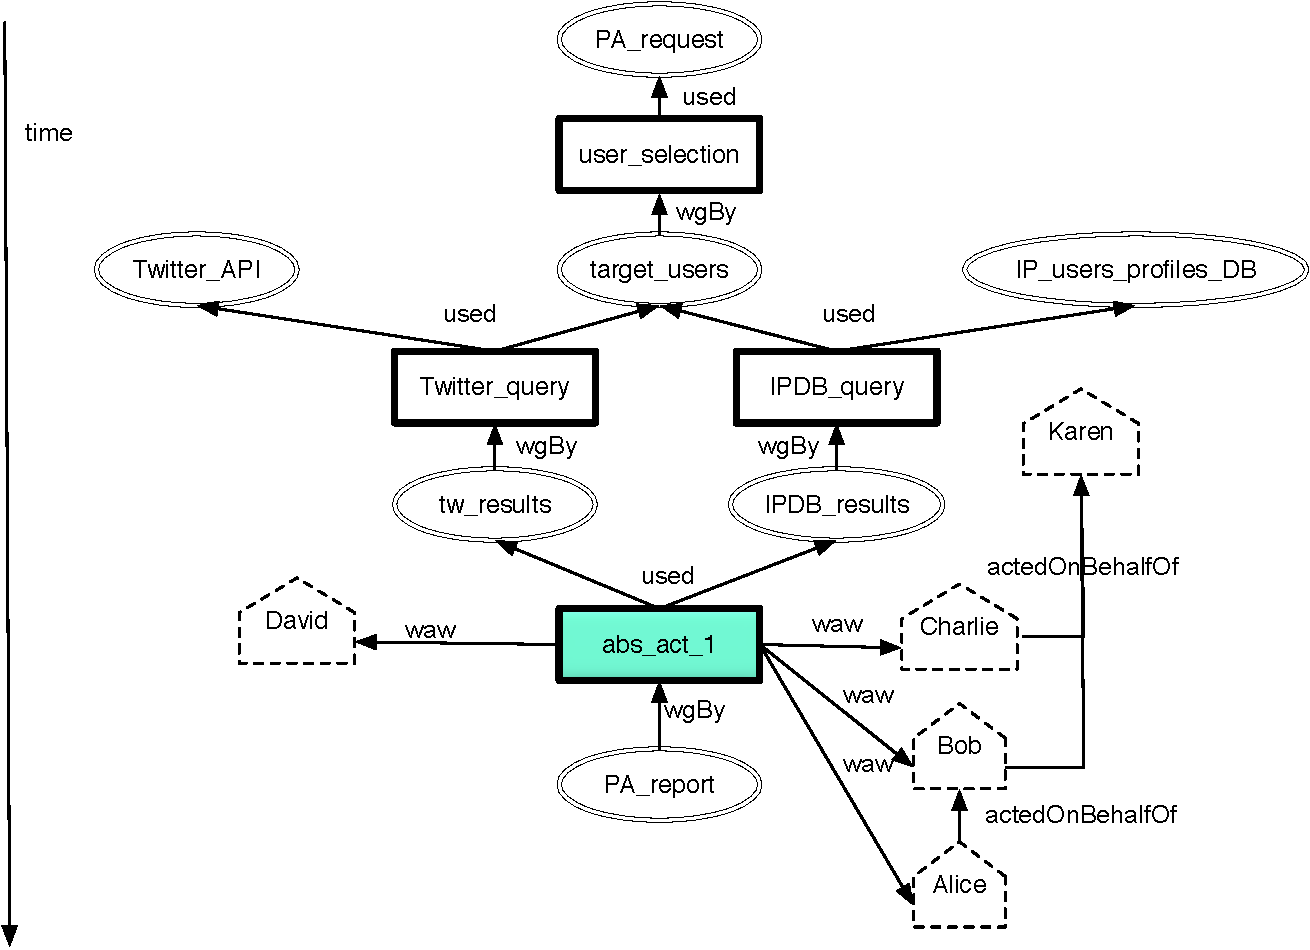
\includegraphics[width=.7\textwidth]{figures/analytics-ex-abs1-FGCS-paper}
			\caption{The result of abstracting out selected nodes \texttt{redact},  \texttt{analytics\_1}, and  \texttt{analytics\_2}  from the graph in Fig.~\ref{fig:graph-example}.} 
			\label{fig:graph-example-abs-1}
		\end{center}
	\end{figure*}	
	
\paolo{By construction, this is a new valid PROV graph. 
It is therefore possible to further abstract out some of its nodes. 
For example, IP may also decide that mentioning the use of a proprietary data source is inappropriate. 
Nodes \texttt{IP\_users\_profiles\_DB} and \texttt{IPDB\_query} are therefore abstracted out. 
As these are both entities, the new abstract node is also an entity, as shown in Fig.~\ref{fig:graph-example-abs-2}.
Note that, to PA, it now appears that the report has been generated from its initial request using Twitter as a data source, and without reference to specific analytics algorithms.
}

	\begin{figure*}
	\begin{center}
		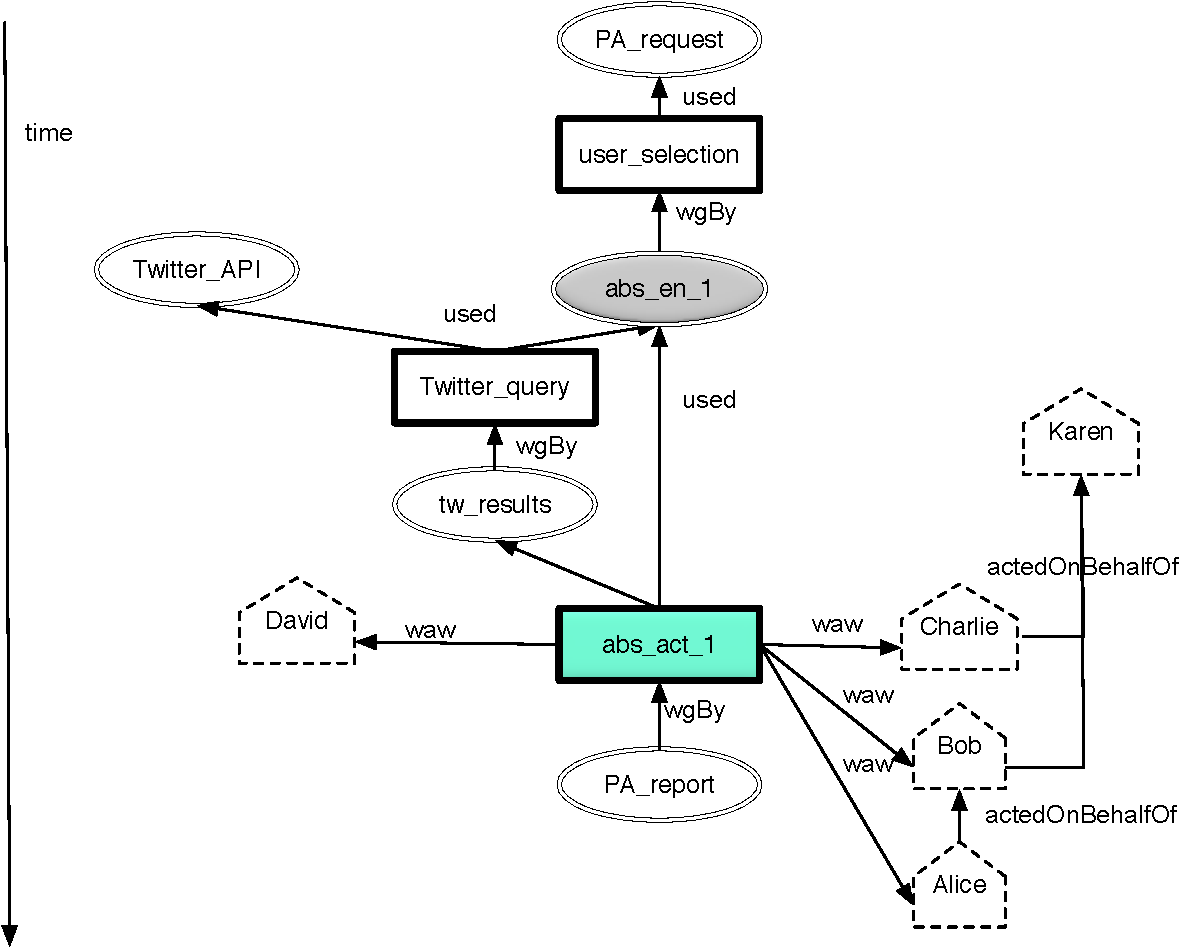
\includegraphics[width=.7\textwidth]{figures/analytics-ex-abs2-FGCS-paper}
		\caption{The result of further abstracting out \texttt{IP\_users\_profiles\_DB} and \texttt{IPDB\_query} after the first abstraction-by-gropuping step (Fig.~\ref{fig:graph-example-abs-1}).} 
		\label{fig:graph-example-abs-2}
	\end{center}
\end{figure*}	

\paolo{The mechanisms by which the data and provenance owner selects the nodes to be abstracted are not discussed in this paper, however a policv-based model is described in detail in our previous work~\citep{MBGCD14,Missier2014}.
	Briefly, the idea, inspired by the Bell-Lapadula model~\citep{bell1996bell},	is that the owner assigns a sensitivity value to each node, and nodes are selected to be abstracted out based on a specific  recipient's clearance level. Thus, different recipients will potentially receive different abstract versions of the same graph.
Note also that forcefully removing nodes that were not marked for abstraction has implications, too, as some of those non-sensitive nodes may have had evidential value that is now lost.
To model this problem we associate a utility value to each node, and compute the \textit{residual utility} of the abstracted graph. 
The papers cited above provide further details.
}

We observe that removal of information from a provenance graph could be achieved in a number of other ways.
%
For example, one could simply remove the labels as well as the annotations from individual nodes and relationships, i.e., anonymize part of the graph. Doing so, however, does not hide any of the structure of the process of data production. One could further remove nodes and relationships or  indeed entire sub-graphs. The new graph will be disconnected, however, making it difficult to reconstruct the lineage of the end data product, that is, the sequence of data derivations from the initial inputs to the outcome of the process.

Instead, our abstraction operator replaces a sub-graph with a new abstract node, and then ``re-wires'' the new node to the remaining original graph. This has the effect of hiding parts of the process structure as it was represented in the original provenance, while maintaining connectivity. One can still query the lineage, but some of the provenance elements returned by the query will now be an abstraction of the actual data production process.

The main challenge is to guarantee that abstraction produces PROV-compliant  graphs,   maintaining the interoperability guarantees provided from having standardized PROV and ensuring that the results can be consumed by standard PROV tools. We provide a proof of this in the Appendix.

\subsection{Contributions} \label{sec:contributions}

In this paper we develop a model and algorithm for performing  abstraction over PROV graphs, providing the theoretical underpinning to ensure that the abstraction process satisfies a number of properties.
%
Our main contribution is the formal definition of a provenance abstraction operator that rewrites  a PROV graph $\pg$ into a new graph $\pg'$, by mapping a set $V_{gr}$ of nodes (for ``vertex in a group'') in $\pg$ to a new abstract node $v_{new}$, and then mapping each relationship involving elements of $V_{gr}$ to a new relationship involving $v_{new}$ in $\pg'$. 
\jwb{The set $V_{gr}$ is chosen by the user of the abstraction operator as the set of nodes she wishes to obfuscate.}

We prove several formal properties of $\pg'$: firstly, schema preservation: if $\pg$ is a PROV graph, that is, it conforms to the PROV data model~\citep{w3c-prov-dm}, then $\pg'$ is also a PROV graph. Secondly, validity preservation: if $\pg$ is \textit{valid}, that is, it satisfies all PROV constraints~\citep{w3c-prov-dm}, then $\pg'$ is also valid. Finally, no spurious dependencies are introduced into $\pg'$: a  relationship involving $v_{new}$ is only created as a result of a mapping from an existing relationship involving elements of $V_{gr}$. Strictly, if $a$ and $e$ are not \textit{directly} related in $\pg$, we guarantee that they are not directly related in $\pg'$. 

Note that new indirect dependencies between two nodes in $\pg'$, manifested as new paths in the graph, may be introduced, however we show that these are always justified by the topology of the underlying graph $\pg$.

Note that, by making the abstraction operator closed with respect to the set of valid PROV graphs, abstraction can be naturally composed, i.e., one can abstract $\pg'$ into some $\pg''$.
%
Finally, note also that $\pg'$ itself has also an associated provenance graph, that is, a record of the provenance abstraction process as it was applied to $\pg$. 
PROV provides a syntactic facility to maintain the association between a provenance graph and its own provenance, namely using the ``provenance of provenance'' mechanism (i.e., bundles~\citep{w3c-prov-dm}).




%
%The remainder of the paper is structured as follows. After a review of related work, in Sec.~\ref{sec:prov-core} we introduce the fragment of the PROV model that defines the scope of our work, followed by an overview of the approach and summary of contributions (Sec.~\ref{sec:overview}).
%%
%The core technical material is in Sec.~\ref{sec:grouping}, where we define abstraction over provenance in terms of a \textit{grouping} operator, present its functional specification, and show that grouping maps a graph into a new graph that conforms to the same relational schema.

